\chapter{付録C NMFのモデルエビデンス}
NMFの基底数を決める際にブートストラップから計算されたモデルエビデンスを用いることを考える.
BICは最尤推定量の尤度からモデルエビデンスを近似して扱っている.
ブートストラップによってモデルエビデンスを近似計算できると考えられる.
本節ではその説明をする.

基底数$k$のNMFのモデルを$\mathcal{M}_k$とおく.
ノイズ行列$H$の各要素が正規分布$\mathcal{N} (0, \sigma^2)$に従う$\mathcal{M}_k$の尤度は以下である.
\begin{align}
	p(X | Y_k, \mathcal{M}_k) = \prod_{i,j} \frac{1}{\sqrt{2 \pi \sigma^2}} \exp(-\frac{([Y_k]_{ij} - x_{ij})^2}{2 \sigma^2}),
\end{align}
ただし,$Y_k = D_k C_k$で,モデル$\mathcal{M}_k$における推定量である.
対数尤度は以下のようになる.
\begin{align}
	\log p(X | Y_k, \mathcal{M}_k) = - \frac{IJ}{2} (\log 2\pi + 2 \log \sigma) - \frac{1}{2 \sigma^2} \sum_{ij}([Y_k]_{ij} - x_{ij})^2.
\end{align}


今回の問題をBayesian model averagingの枠組みに当てはめると,
\begin{align}
	p(A|X) = \sum_k p(A|\mathcal{M}_k, X) p(\mathcal{M}_k | X)
\end{align}
で$p(A|X)$を求めることになる.
今回は異なる基底数のNMFから求まった$A$をモデルの事後確率で重み付けて足し合わせることになる.

モデルの事後確率は
\begin{align}
	p(\mathcal{M}_k|X) = \frac{m_k p(\mathcal{M}_k)}{\sum_l m_l p(M_l)}
\end{align}
で表される.
ただし,
\begin{align}
	m_k = \int p(X | Y_k, \mathcal{M}_k) p(Y_k| \mathcal{M}_k) dY_k
	\label{eq:evidence}
\end{align}
である.
これはモデルエビデンスやmarginal likelihoodと呼ばれる.
また,$p(\mathcal{M}_k)$はモデルが正しい確率である.

ある条件下で,母数の事後確率の密度関数はブートストラップによる最尤推定量の分布と同じになる.
そのため,ブートストラップサンプルから推定した$A$の分布をもとに事後確率を計算すれば良い.

現在の設定では$p(\mathcal{M}_k)$は一様なため,エビデンスを見る必要がある.

\subsection{ラプラス近似}
エビデンスの計算には事前分布を決めなければならず,積分も計算しなければいけない.
そこでラプラス近似により$m_k$は以下のような$\hat{m_k}$で近似できる.
\begin{align}
	\log \hat{m}_k = \log p(X | \hat{Y_k}, \mathcal{M}_k) - \frac{d_k}{2} \log n
	\label{eq:simm}
\end{align}
ここで,$d_k$は母数の数($I \times K + K \times J$),$n$は観測データ数($J$)である.
この近似を使ってBayes因子のログを計算したのがBICである.
Bayes因子は2つのモデルエビデンスの比である.

$\log p(X | \hat{Y_k}, \mathcal{M}_k)$は初期値を変えてNMFを行い,尤度が最も大きくなった対数尤度を用いる.
また,$\sigma^2 = Var(X - Y_k)$として計算する.

\subsection{ブートストラップによる近似}
ブートストラップの推定量の分布は最尤推定量の分布を近似する(ブートストラップサンプルが生成されたパラメータ分バイアスは乗る)ので,$m_k$は以下のように近似できる.

\begin{align}
	m_k &= \int p(X | Y_k, \mathcal{M}_k) p(Y_k| \mathcal{M}_k) dY_k \\
	&\sim \frac{1}{B} \sum_b \prod_{i,j} \frac{1}{\sqrt{2 \pi \sigma^2}} \exp\left(-\frac{([Y_k^b]_{ij} - X^b_{ij})^2}{2 \sigma^2} \right) \\
	\label{eq:simm2}
\end{align}

ここで,$Y_k^b$はブートストラップサンプル$b$から計算された$Y_k$で,$B$はブートストラップサンプル数である.
また,$\sigma^2 = Var(X^b - Y^b_k)$として計算する.

\subsection{実験}
人工データセット86個について2つの近似方法でモデルエビデンスを計算した.
その結果を\Figref{fig:evidence1}と\Figref{fig:evidence2}に示す.
同じデータの結果を線で結んでいる.
ラプラス近似を行った場合は真の基底数10付近で最大値をとっている.
ブートストラップによる近似を行った場合は基底数に比例してエビデンスの値も大きくなっている.
また,同じデータでも基底数によってオーダーが大きく異なるが,これは尤度計算に用いる分散をデータから計算しているためである.

\begin{figure}[htbp]
    \begin{minipage}{0.5\hsize}
			\begin{center}
					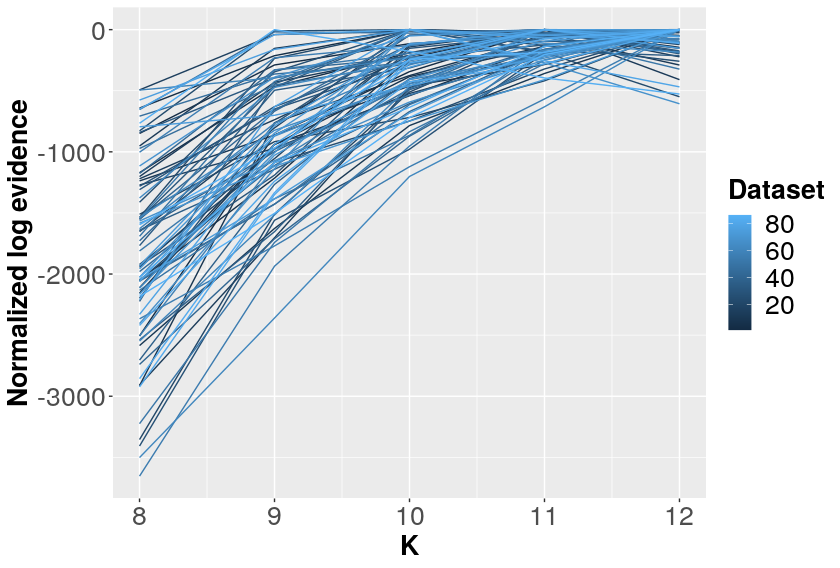
\includegraphics[width=\hsize]{evidence1log}
					\caption{ラプラス近似によって計算されたログエビデンス.各データについて最大値が0となるように定数を足した.}
					\label{fig:evidence1}
			\end{center}
		\end{minipage}
    \begin{minipage}{0.5\hsize}
			\begin{center}
					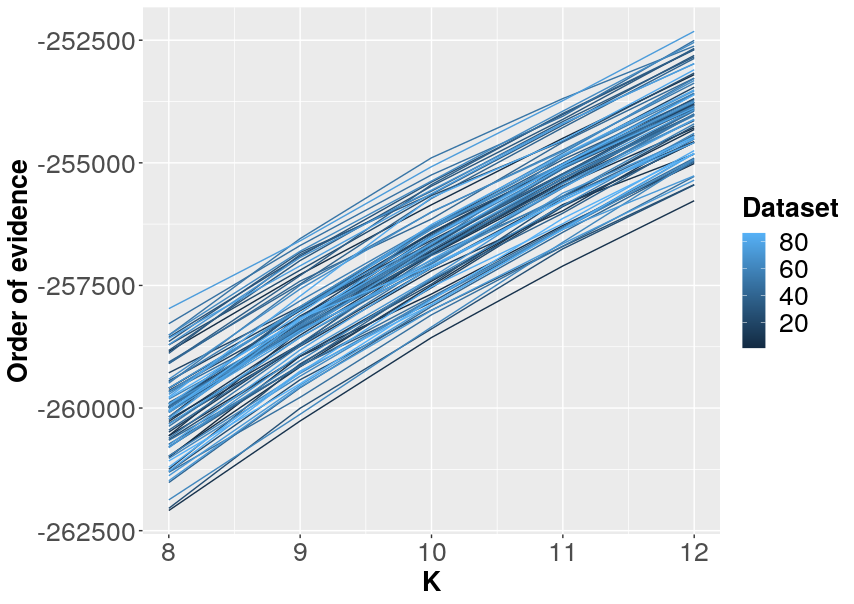
\includegraphics[width=\hsize]{evidence2order}
					\caption{ブートストラップ近似によって計算されたエビデンスのオーダー(10を底とした指数).}
					\label{fig:evidence2}
			\end{center}
		\end{minipage}
\end{figure}

また,\Figref{fig:evidence2}のログを取り,\Figref{fig:evidence1}とプロットした図を\Figref{fig:evidence12}に示す.
これより,ブートストラップによる近似を用いた場合のエビデンスの値は大きいことが分かる.
ラプラス近似では$\frac{d_k}{2} \log n$によって補正された値である.
NMFではデータが増えると補正の値も増えるためラプラス近似は適さないが,\Figref{fig:evidence12}の2つの近似手法のエビデンスの差が過剰に足された補正の値だとも考えることができる.

\begin{figure}[htbp]
    \begin{center}
        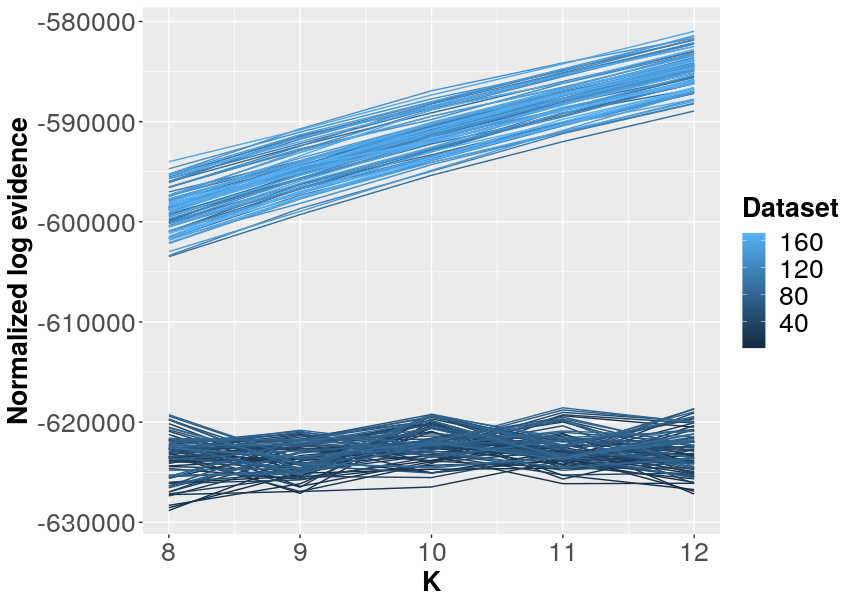
\includegraphics[width=0.8\linewidth]{evidence12log}
        \caption{2つの近似方法によって計算されたログエビデンス.}
        \label{fig:evidence12}
    \end{center}
\end{figure}
